    \section{Graphical User Interface}

        Die GUI wird mit dem Qt-Framework umgesetzt, wobei grafische Elemente im Besonderen mit QML implementiert werden. Dies unterstützt die strikte Trennung von Präsentation, Steuerung und Struktur der zugrundeliegenden Daten.

        Die Kommunikation mit dem \textit{Core} erfolgt über eine C++-Schnittstelle auf Basis des Observer-Patterns.


        \subsection{Fenstermanagement}

            Die GUI soll aus verschiedenen Modulen bestehen, die zunächst als Editor-, Register-, Speicher-, Projekt-, Hilfs- und Output-Modul identifiziert wurden. Die darüberliegende Toolbar steuert Abläufe und Einstellungen, die über Modulgrenzen hinweg Relevanz haben.

            Die Unterbringung der Module erfolgt in einem tabellarischen Layout bestehend aus 4 Spalten zu je 1 bis 2 Zeilen. Die untere Zeile einer Spalte kann je nach Bedarf angezeigt oder ausgeblendet werden.

            Die dadurch entstehenden Modulzellen sollen variabel mit den oben beschriebenen Modulen belegt werden können, was die Möglichkeit mit einschließt, ein Modul mehrfach in verschiedenen Zellen anzuzeigen. Ein einfaches Anwendungsbeispiel für dieses Feature ist das parallele Arbeiten auf zwei Bereichen den Speichers.

		    \begin{figure}
		    	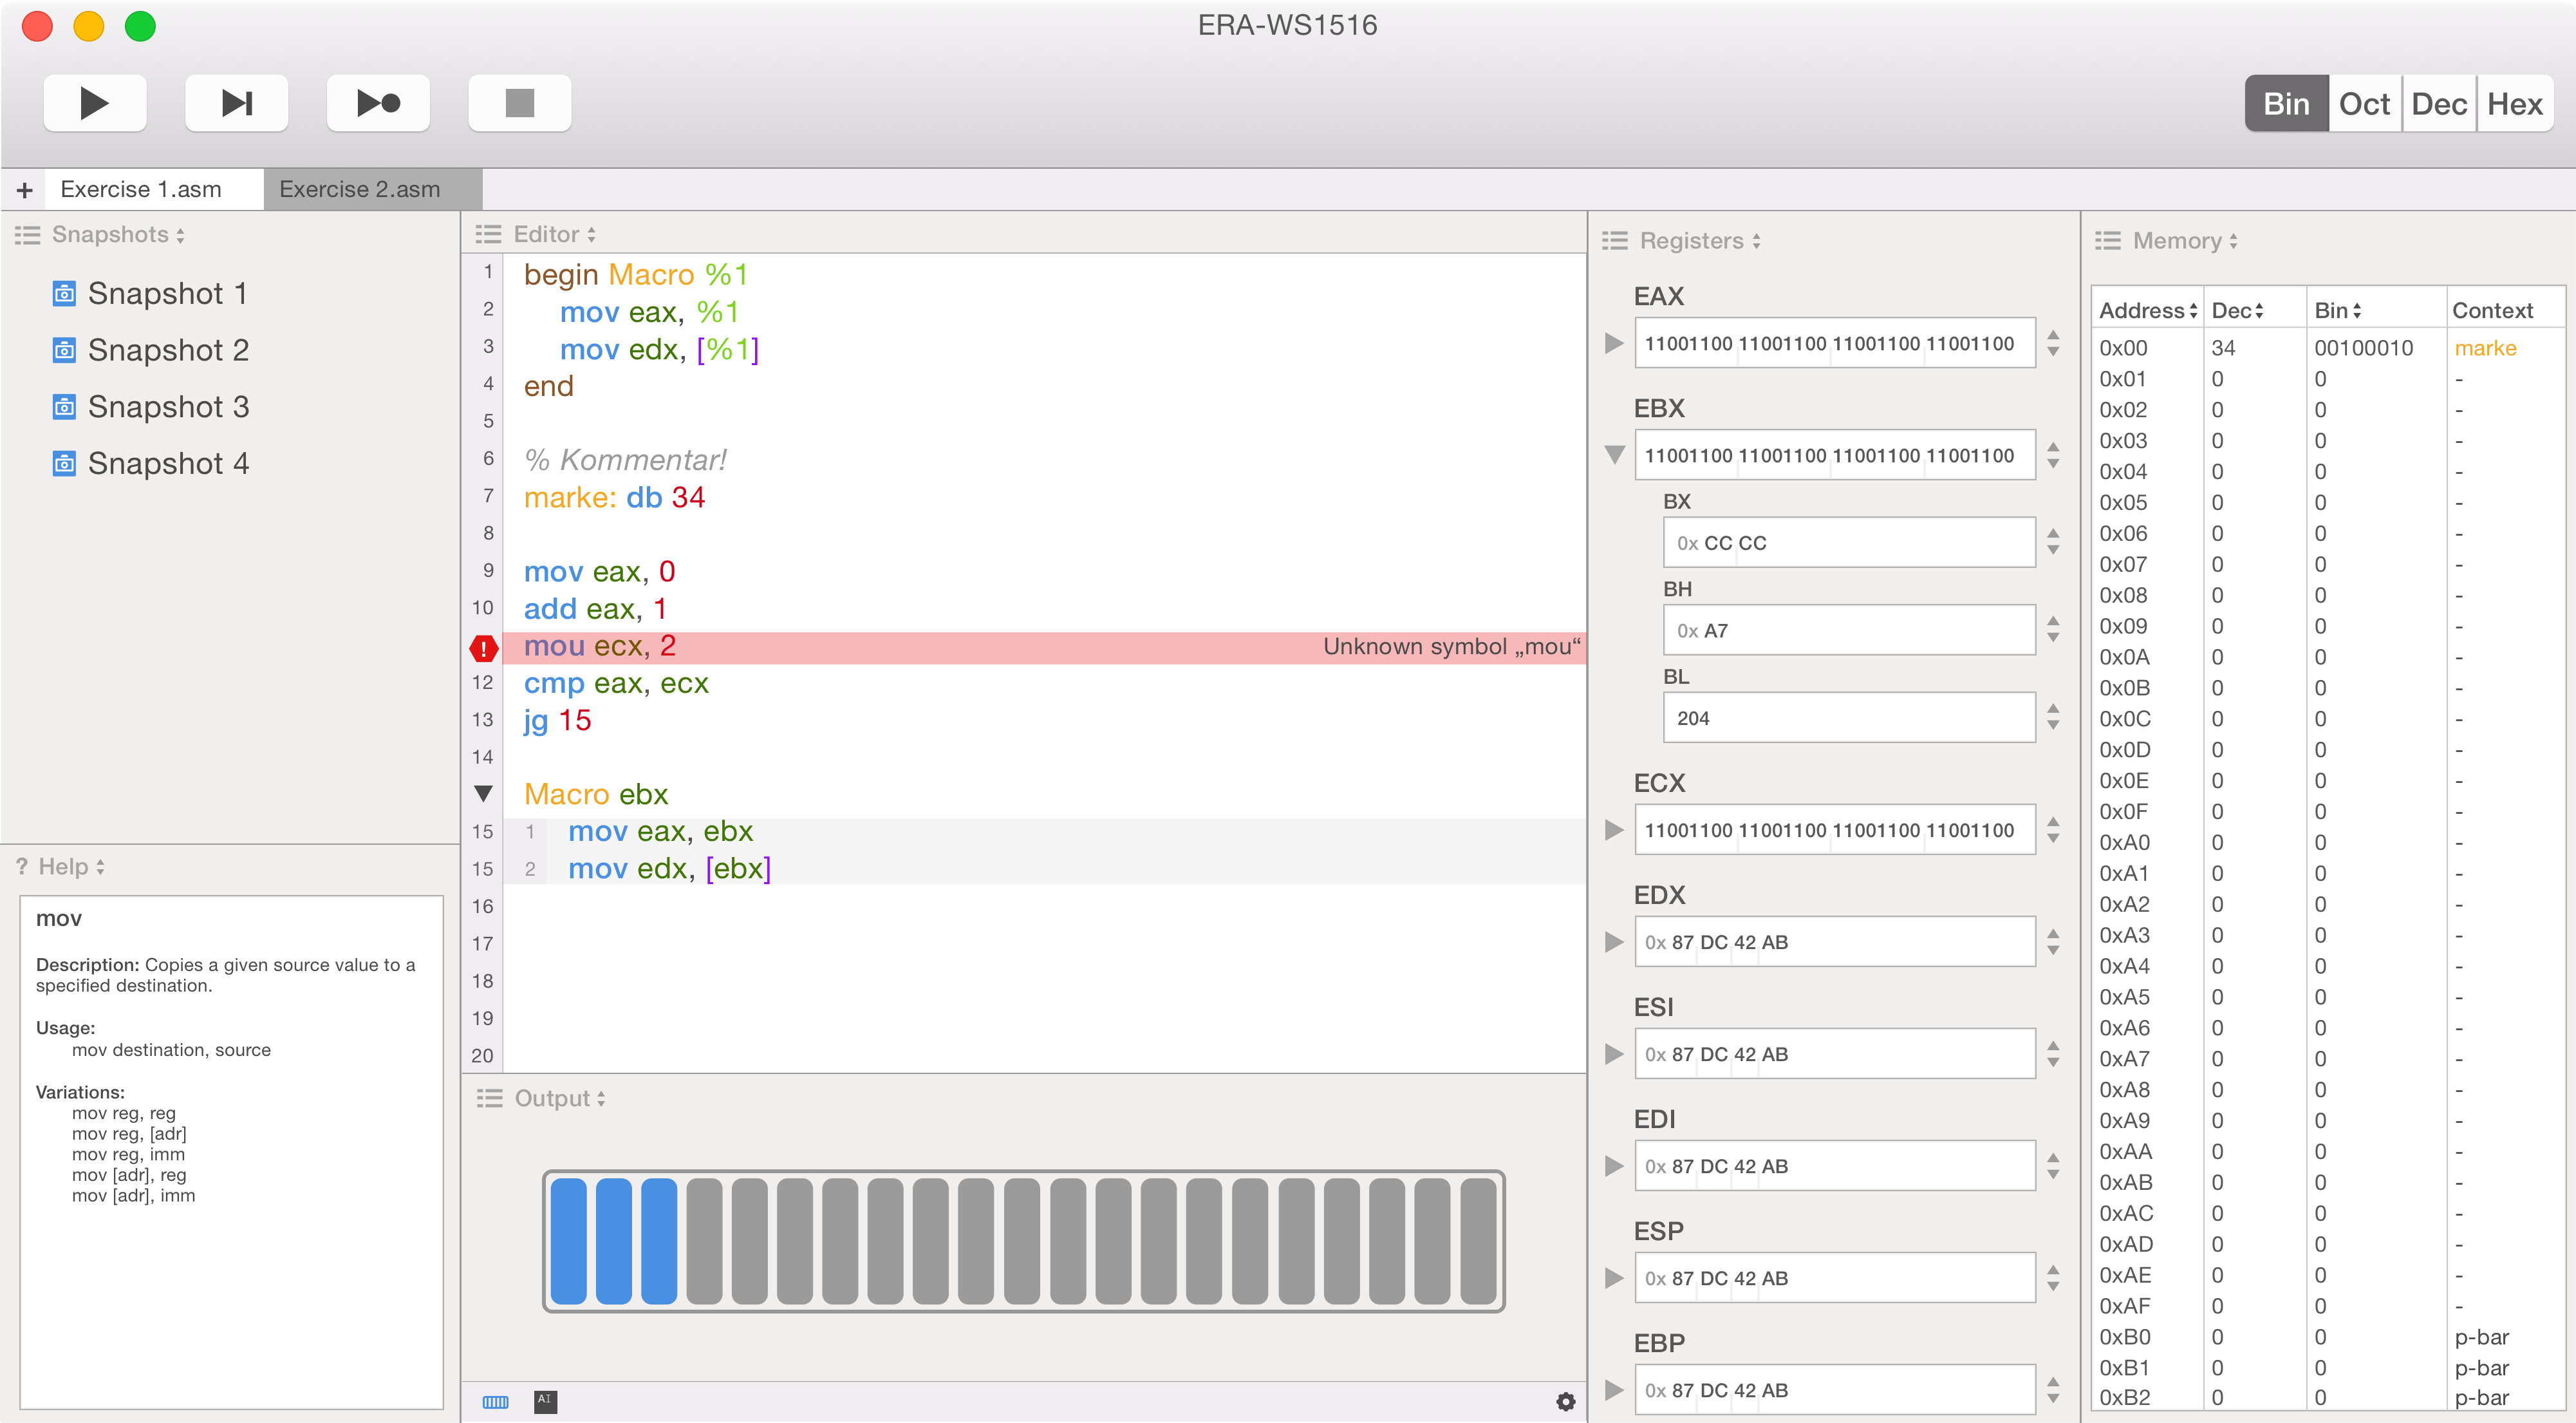
\includegraphics[width=\textwidth]{../ui/figures/mockup}
		    	\label{fig:Mockup}
		    	\caption{Der obige rein visuelle Entwurf soll einen groben Überblick über die geplante Umsetzung der Benutzeroberfläche geben. Im Wesentlichen ist die Aufteilung des Fensters in Toolbar und die vier Spalten mit ein bis zwei Zeilen erkennbar. Zudem wurden die einzelnen Module skizziert.}
		    \end{figure}

        \subsection{Toolbar}

            Über die Toolbar kann die \textbf{Ausführung} des Programms gesteuert werden, wobei die Optionen \textit{Ausführung des gesamten Programms}, \textit{Ausführung einer einzelnen Instruktion}, \textit{Ausführung bis zum nächsten Breakpoint} und \textit{Abbrechen der Programmausführung} zur Verfügung stehen.

            Des Weiteren lässt sich das \textbf{Zahlenformat} modulübergreifend festlegen, was insebesondere Einfluss auf Register- und Speicherinhalte hat.

        \subsection{Editor}

            Der Editor für die Eingabe der Assembler-Instruktion soll \textbf{Syntax-Highlighting} unterstützen, um Instruktions-Komponenten visuell zu trennen. Die Umsetzung erfolgt mit dem Qt-eigenen Syntax-Highlighter (\textit{QHighlighter}), welcher mit Regex-Ausdrücken initialisiert wird. Diese werden vom Parser in Kombination mit Architektur-eigenen Keywords generiert und über den Core zur Verfügung gestellt.

            \textbf{Fehlermeldungen}, die vom Parser ermittelt wurden, werden innerhalb der zugehörigen Zeile im Editor angezeigt, was es ermöglicht mehrere Fehlermeldungen gleichzeitig anzuzeigen.

            Ein \textbf{Makroaufruf} wird im Editor als einzelne Zeile dargestellt, die bei Bedarf vom User aufgeklappt werden kann, wodurch die Makrodefinition in-place eingeblendet wird. Dies ermöglicht u.a. die schrittweise Ausführung des Codes.

        \subsection{Register}

            Die Registerwerte werden übersichtlich mit Hilfe von Byte-Separatoren dargestellt. Zu den jeweiligen Registern gehörige Unterregister können separat eingeblendet werden.

            Registern wie Unterregistern kann unabhängig von den globalen Einstellungen ein eigenes Zahlenformat (binär, hexadezimal etc.) zugewiesen werden.

            Intern werden die einzelnen Zahlenformate vom \textit{Core} berechnet und als String an die GUI übergeben.

        \subsection{Speicher}

            Der Speicher teilt sich in drei Hauptbereiche: Speicheradressen, Speicherinhalte und Kontextinformationen.

            Der \textbf{Adressraum} erlaubt die Unterteilung in verschiedene Datenformate, darunter Byte, Halbwort, Wort etc.

            Das Zahlenformat der \textbf{Speicherinhalte} ist spaltenweise anpassbar.

            \textbf{Kontextinformationen} zu einzelnen Speicherzellen geben Hinweise auf die Verwendung im Programm, darunter etwa Marken zu Datendefinitionen, Speicherbereiche für Ausgabegeräte und Speicher-Referenzierungen durch Register.

        \subsection{Projekt}

            Das Projekt-Modul dient der \textbf{Datei-Verwaltung}. Gegebenefalls können ein oder mehrere Dateien zu Projekten zusammengefasst werden, welche dann zusätzliche Information etwa über die verwendete Architektur sowie Speicher- und Registerinhalte speichern können.